%
% main.tex -- Paper zum Thema visuell
%
% (c) 2019 Hochschule Rapperswil
%
\chapter{Gabor-Wavelets und visuelle Wahrnehmung\label{chapter:visuell}}
\lhead{Gabor-Wavelets und visuelle Wahrnehmung}
\begin{refsection}
\chapterauthor{Raphael Unterer}

\section{Einleitung}
\rhead{Einleitung}

Die visuelle Wahrnehmung des Menschen ist spezialisiert auf das Erkennen von Mustern und Objekten.
\index{visuelle Wahrnehmung}%
Bilder vom menschlichen Auge werden im visuellen Kortex 1 vorverarbeitet.
\index{Auge}%
\index{visueller Kortex 1}%
Diese Vorverarbeitung kann mit Hilfe von 2-dimensionalen Gabor-Wavelets modelliert werden.

Viele Probleme im Bereich des maschinellen Lernens versuchen ebenfalls Objekte in Bildern zu erkennen.
Vor allem Convolutional Neural Networks (CNN) zeigen gute Ergebnisse.
\index{Convolutional Neural Network}%
\index{CNN}
Dementsprechend wäre es interessant zu Wissen, ob mit einer Gabor-Wavelet Vorverarbeitung eine Verbesserung der CNNs erreicht werden kann.

Das Ziel dieses Papers ist es, alle diese Dinge (Gabor-Wavelets, Neurologie und CNNs) genauer zu analysieren.
Abschliessend wird in einem Experiment gezeigt, inwiefern eine Gabor-Wavelet-Transformation als Vorverarbeitung Sinn macht.
\index{Neurologie}


\section{Zweidimensionales Gabor-Wavelet}
\rhead{Zweidimensionales Gabor-Wavelet}

Die Idee des eindimensionalen Gabor-Wavelets wird zuerst als Grundlage genommen. 
Daraus wird dann das zweidimensionale Wavelet abgeleitet und die entstehenden Freiheitsgrade erläutert.

\subsection{Gabor-Wavelet}

Bei der Wavelet-Transformation besteht eine Zeit-Frequenz-Unschärfe.
Diese Unschärfe bewirkt, dass die Auflösung im Zeitbereich umgekehrt proportional zur Auflösung im Frequenzbereich ist.
Das Gabor-Wavelet stellt einen optimalen Kompromiss aus Zeit-und Frequenzauflösung dar.
Die Anwendung des Wavelets minimiert dabei das Produkt der Standardabweichungen im Zeit- und Frequenzbereich. \cite{paper:communication}
%TODO more details?

Ein solches Gabor-Wavelet besteht aus einer komplexen Schwingung, welche mit einer Gaussfunktion gefenstert ist und somit exponentiell abfällt.

\begin{equation}
G(x)= e^{-\frac{(x-x_{0})^{2}}{\sigma^{2}}} e^{i\xi_{0}x}
\end{equation}

Der Parameter $\sigma$ beschreibt die Standardabweichung der Gaussfunktion und $\xi$ die Frequenz der komplexen Schwingung. 
Die komplexe Schwingung besteht aus einem Sinus und einem  Kosinus Anteil. 
Ein Beispiel eines Sinus-Gabor-Wavelet wird in Abbildung \ref{fig:gabor1d} gezeigt.

\begin{figure}
	\centering
	\includegraphics[width=0.7\linewidth]{./papers/visuell/images/gabor_1d}
	\caption{Beispiel eines Sinus-Gabor-Wavelets}
	\label{fig:gabor1d}
\end{figure}


\subsection{Erweiterung auf zwei Dimensionen}

Um ein solches Wavelet auf ein Bild anwenden zu können, ist es sinnvoll dieses auf zwei Dimensionen zu erweitern.
Diese Erweiterung ergibt die folgende Formel:

\begin{equation}
G(x,y)= e^{-(\frac{(x-x_{0})^{2}}{\sigma^{2}}+\frac{(y-y_{0})^{2}}{\beta^{2}})}
e^{i(\xi_{0}x+\nu_{0}y)}.
\end{equation}

Das zweidimensionale Wavelet besteht immer noch aus einer komplexen Schwingung multipliziert mit einer elliptischen Gaussfunktion. 
Diese Schwingung kann man sich als ebene Welle vorstellen, welche abhängig von $\xi$ und $\nu$ in eine bestimmte Richtung zeigt (vgl. Abbildung \ref{fig:planarwave}).

\begin{figure}
	\centering
	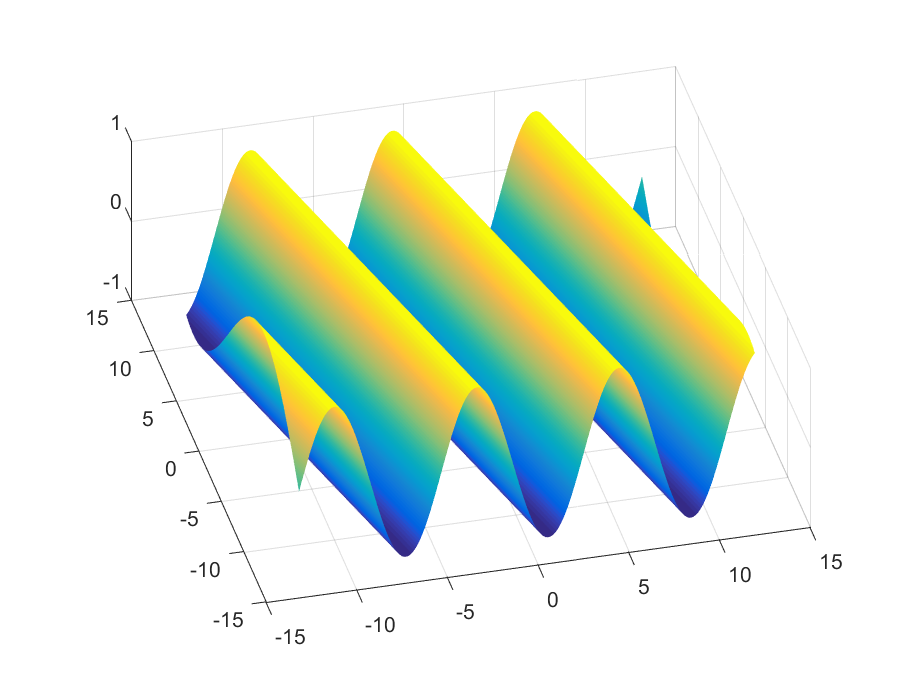
\includegraphics[width=0.7\linewidth]{./papers/visuell/images/planarwave.eps}
	\caption{Beispiel einer ebenen Welle}
	\label{fig:planarwave}
\end{figure}



Diese Parameter ($\sigma$, $\beta$, $\xi$, $\nu$) dieser Formel sind unhandlich und es ist nicht offensichtlich was eine Änderung dieser bewirkt.
Also ersetzen wir diese durch neue Parameter und erhalten 

\begin{equation}
G(x,y)=e^{-\frac{x'^{2}+\gamma^{2}y'^{2}}{2\sigma^{2}}}
e^{i(2\pi\frac{x'}{\lambda} + \phi)},
\end{equation} 
wobei $x'=x\cos(\theta)+y\sin(\theta)$ und $y'=-x\sin(\theta)+y\cos(\theta)$.
Der Parameter $\gamma$ beschreibt das Verhältnis der Streckung in $x$- und $y$-Richtung.
Diese Streckung der elliptischen Gaussfunktion bestimmt ob das Wavelet eher rund oder länglich ist.
Die Standardabweichung der Gausskurve welche mit der Schwingung multipliziert wird ist als Parameter $\sigma$ definiert.
Grösseres $\sigma$ bewirkt ein breiteres Wavelet.
Die komplexe Schwingung wird durch die Wellenlänge $\lambda$ und die Phase $\phi$ definiert.
Der Parameter $\theta$ definiert nun die Ausrichtung der komplexen Schwingung.
Eine Änderung von $\theta$  bewirkt somit eine Drehung der Wellenfronten.

Wie sich Gabor-Wavelets in Abhängigkeit dieser Parameter Verhalten zeigt Abbildung \ref{fig:kernels}.

\begin{figure}
	\centering
	\subfigure[Parameter der Gaussfunktion $\gamma$ und $\sigma$ werden verändert]{\label{fig:kernels_a}\includegraphics[width=0.45\linewidth]{./papers/visuell/images/kernels_sigma_gamma.pdf}}
	
	\subfigure[Wellenlänge der Schwingung $\lambda$ und Ausrichtung $\theta$ werden verändert]{\label{fig:kernels_b}\includegraphics[width=0.45\linewidth]{./papers/visuell/images/kernels_theta_lambda.pdf}}
	\caption{Abhängigkeit des Gabor-Wavelets von den Parametern}
	\label{fig:kernels}
\end{figure}

\section{Visuelle Wahrnehmung}
\rhead{Visuelle Wahrnehmung}

In den vorherigen Abschnitten haben wir das zweidimensionale Gabor-Wavelet genauer betrachtet.
Dieses Wavelet ist einerseits der optimale Kompromiss zwischen Zeit- und Frequenzauflösung und andererseits kann es in verschiedene Richtungen ausgerichtet werden.
Diese speziellen Eigenschaften sind sehr nützlich und es zeigte sich, dass die Hirne von Säugetieren ähnliche Eigenschaften besitzen.
In den folgenden Abschnitten wird versucht zu zeigen was die visuelle Wahrnehmung und Gabor-Wavelets gemeinsam haben. 

\subsection{Primärer Visueller Kortex}\label{subsec:v1}

Der primäre Visuelle Kortex (V1) verarbeitet die Bildinformationen welche vom Auge aufgenommen werden.
Als Ausgangsprodukt stellt er abstrakte Features zu Verfügung, welche dann vom Hirn zusammen mit weiteren Informationen (Kontextwissen, andere Sinne)  benützt werden, um Objekte zu erkennen.
Erste Analysen des V1 wurden von Hubel und Wiesel bereits 1959 veröffentlicht \cite{paper:hubelwiesel}.
Ihre Erkenntnisse haben sie anhand von Versuchen an Katzenhirnen gewonnen.

Jedes Neuron innerhalb des V1 bekommt Eingangssignale einer bestimmten Region der Netzhaut.
Eine solche Region wird rezeptives Feld genannt.
Diese rezeptiven Felder bestimmen also welcher Teil eines Bildes vom Neutron bearbeitet wird.
Es gibt verschiedene Arten von Neuronen innerhalb des V1.
Eine wichtige Gruppe davon die die sogenannten einfachen Zellen.
Diese zeigen ein orientierungsspezifisches Antwortverhalten auf optische Inputs.
Ausserdem beinhalten die einfachen Zellen immer abwechselnde ON und OFF Regionen, welche ansprechen bei Licht (ON) oder eben keinem Licht (OFF).
Die zweite wichtige Gruppe der Neuronen sind die komplexen Zellen.
Diese können als Kombination von mehreren einfachen Zellen modelliert werden, wobei alle einfachen Zellen in die selbe Richtung orientiert sind.
Allerdings ist diese Erklärung der komplexen Zellen nicht überall anerkannt \cite{book:neuroscience}.


\subsection{Modellierung der Funktion des V1 mithilfe von Gabor-Wavelets}

Die Eigenschaften der einfachen Zellen sind sehr ähnlich derjenigen des Gabor-Wavelets.
Deshalb haben Forscher begonnen die einfachen Zellen mithilfe von Gabor-Wavelets zu modellieren \cite{paper:imgrep}.
Analog zu den einfachen Zellen können Gabor-Wavelets ebenfalls in beliebige Richtungen ausgerichtet und deren Wellenlänge variiert werden.
Ausserdem kann die Schwingung des Gabor-Wavelets als ON-OFF-Pattern interpretiert werden.
Dies ist eine sehr schöne Entdeckung, da es zeigt, dass sich der V1 während der Evolution hin zu einem optimalen Kompromiss aus Zeit- und Frequenzinformationen entwickelt hat.
Die Eigenschaften des Gabor-Wavelets sollten auch für die künstliche Bilderkennung sinnvoll sein, da es offensichtlich einen evolutionären Vorteil darstellt wenn Bilder in dieser Art vorverarbeitet werden.
\section{Künstliches Neuronales Netz}
\rhead{Künstliches Neuronales Netz}

Künstliche neuronale Netze (KNN) stellen eine Möglichkeit des maschinellen Lernens dar, welche vom Hirn inspiriert wurde.
Ein KNN besteht aus verschiedenen Neuronen, welche Hierarchisch (in sogenannten Layern) angeordnet werden (vgl. Abbildung). %TODO Abbildung KNN
Jeder Eingangswert $x_i$ zu einem Neuron wird mit einem Faktor $w_i$ multipliziert.
Alle gewichteten Eingänge werden zusammen mit einem Schwellenwert $b$ addiert.
Diese Summe wird danach durch eine nichtlineare Aktivierungsfunktion $H$ aktiviert und bildet so den Ausgang $y$
\begin{equation}
y=H((\sum_{i} x_i w_i)+b).
\end{equation}
Die Nichtlinearität ist entscheidend um nichtlineare Probleme lösen zu können.
der Aufbau eines Neuron ist in Abbildung gezeigt. %TODO Abbildung Neuron

\subsection{Convolutional Neural Nets}

Eine Unterkategorie der KNNs stellen die Convolutional Neural Nets (CNN) dar.
Wie der Name schon sagt spielen dabei Faltungen eine wichtige Rolle.
Bevor die normalen KNN Layer kommen, werden Bilddaten üblicherweise zuerst von einigen Faltungslayern vorverarbeitet.
Die Idee dazu kommt von der klassischen Bildverarbeitung, wo häufig Faltungskernel verwendet werden um ein Bild zu filtern oder Features zu erkennen.
Bei einem CNN werden diese Kernel nicht vom Ingenieur bestimmt, sondern während Trainings durch den Algorithmus gelernt.  %TODO insert 2D-Conv image?
Solche CNNs zeigen extrem gute Resultate in der Bildverarbeitung, speziell im Bereich der Klassifizierung von Bildern (z.B. Erkennen von Katzen).

Die zweidimensionale Wavelet-Transformation kann auch als Faltung des Bildes mit dem Kernel (Wavelet) interpretiert werden.
Dabei werden allerdings nicht mehr alle kontinuierlichen Grössen des Wavelets berücksichtigt, sondern nur noch eine diskrete Anzahl.
Da KNNs (und CNNs) vom Hirn inspirierte Algorithmen darstellen und die Bildvorverarbeitung im Hirn als Gabor-Wavelet-Transformation modelliert werden kann, drängt sich daher eine Kombination dieser beiden Konzepte auf.

Eine offensichtliche Idee ist dabei das Vorverabeiten der Bilder mithilfe von Gabor-Wavelets.
Diese vorverarbeiteten Bilder können dann als Input in das CNN verwendet werden und sollten gute Resultate zeigen, analog zum menschlichen Hirn.
Ein Versuch dieses Konzept auszuführen wird in den nächsten Abschnitten erläutert. %TODO insert image of concept?

\subsection{Versuch}


\section{Resultate}
\rhead{Resultate}

Die Ergebnisse des Versuches sind erstaunlich eindeutig.
Die Variante mit Gabor-Kerneln erreicht immer höhere Genauigkeiten als die klassische CNN Variante.
Gleichzeitig müssen bei der Gabor Variante weniger Gewichte gelernt werden, weshalb die Trainingszeit reduziert wird.
Also werden nicht nur bessere Resultate erreicht, es werden auch noch weniger Ressourcen für das Training benötigt.

In Abbildung \ref{fig:acc} sind die Genauigkeiten der beiden Varianten über fünf Trainingsepochen gezeigt.
Eine Epoche entspricht dabei einem kompletten Trainingsdurchgang durch den gesamten Trainingsdatensatz.
Beide Varianten sind 10 mal trainiert worden. 
Es zeigt sich das die Variante mit dem fixen Gabor-Layer in allen 10 Fällen eine höhere Genauigkeit aufweist.
Die kleinste Genauigkeit der Gabor-Variante nach 5 Epochen beträgt 67.32\% und die höchste Genauigkeit der klassischen Variante 66.42\%.
Somit haben wir eine Lücke zwischen den beiden Varianten von ca. 1\%.
Falls über eine längere Zeit trainiert wird (z.B. 20 Epochen), verändern sich die Resultate nur minimal und der Unterschied der beiden Varianten bleibt bestehen.
Unsere Resultate bestätigen also die Hypothese \ref{hyp:1}.

\begin{figure}
	\centering
	\includegraphics[width=0.7\linewidth]{./papers/visuell/images/accuracy}
	\caption{Test-Genauigkeit (Accuracy) der beiden Varianten im Laufe des Trainings.}
	\label{fig:acc}
\end{figure}

Entscheidend bei neuronalen Netzen sind neben der Genauigkeit die Geschwindigkeiten für das Trainieren und das Klassifizieren.
Bei der Variante mit Gabor dauerte das Training etwa 3 Minuten und 10 Sekunden (kann abhängig vom Computer und Grafikkarte stark variieren).
Bei der zweiten Variante, wo erste Layer ebenfalls gelernt wird, dauert das Training ca. 15\% länger (also etwa 3 Minuten und 38 Sekunden).
Das Klassifizieren von neuen Bildern dauert danach bei beiden Varianten gleich lange, da in beiden Fällen die identische Tensorflow-Struktur implementiert wurde.

Lernt das klassische CNN Kernels welche Ähnlichkeiten zu Gabor-Wavelets aufweisen?
In unserem Versuch ist dies nicht der Fall.
Die Kernel welche gelernt wurden sehen zufällig aus, es sind keine Regelmässigkeiten zu erkennen (vgl. Abbildung \ref{fig:cnnkernels}).
Durch die zufällige Initialisierung ist es aber nicht ausgeschlossen dass solche Gabor-Ähnlichen Kernels gelernt werden könnten.
Es gibt genügend Beispiele wo Kernels gelernt wurden, welche gewisse Ähnlichkeiten zu Gabor-Kerneln aufweisen (z.B. im Paper \cite{paper:cifar10}).

\begin{figure}
	\centering
	\subfigure{\includegraphics[width=0.3\linewidth]{./papers/visuell/images/kernel1}}
	\subfigure{\includegraphics[width=0.3\linewidth]{./papers/visuell/images/kernel2}}
	\subfigure{\includegraphics[width=0.3\linewidth]{./papers/visuell/images/kernel3}}
	\caption{Drei verschiedene Kernels des ersten Layers welche vom Netzwerk gelernt wurden. Es sind keine Regelmässigkeiten erkennbar.}
	\label{fig:cnnkernels}
\end{figure}


\section{Schlussfolgerung}
\rhead{Schlussfolgerung}

In den vorherigen Abschnitten haben wir gezeigt, wie Gabor-Wavelets zur Verbesserung von CNNs im Bereich Bildklassifizierung genutzt werden können.
Die Motivation zu diesem Schritt kommt aus der Neurologie, wo mithilfe von Gabor-Wavelets die Funktionsweise von einfachen Zellen im primären Visuellen Kortex modelliert wird.
Der Versuch hat an einem praktischen Beispiel gezeigt, wie mit einer simplen Gabor-Vorverarbeitung die Genauigkeit von einem CNN verbessert werden kann.
Diese Verbesserung konnte erreicht werden ohne die Rechenleistung für Klassifizierungen zu erhöhen, und beim Trainieren genügt sogar eine kleinere Rechenleistung.
Auf Grund dieser Erkenntnisse drängt sich eine solche Vorverarbeitung bei vielen Problemen des maschinellen Lernens auf. 

Natürlich können diese Gabor-Ideen noch auf viele andere Arten implementiert werden.
Eine logische Erweiterung dieser Arbeit wäre es zum Beispiel, die Parameter der zweidimensionalen Gabor-Wavelets während des Trainings automatisiert zu lernen.


\printbibliography[heading=subbibliography]
\end{refsection}
